%~~~~~~~~~~~~~~~~~~~~~~~~~~~~~~~~~~~~~~~~~~~~~~~~~~~~~~~~~~~~~~~~~~~~~
%
%    File       : metodologia
%    Type       : TeX
%    Date       : terça-feira, março 19, 2012 at 10:32
%
%    Content 	: Metodologia utilizada para esta pesquisa
%~~~~~~~~~~~~~~~~~~~~~~~~~~~~~~~~~~~~~~~~~~~~~~~~~~~~~~~~~~~~~~~~~~~~~

%---------------------------------------------------------------------
\chapter{Metodologia}\label{metodologia}
%---------------------------------------------------------------------

%---------------------------------------------------------------------
\section{Tipo e classificação da pesquisa}
%---------------------------------------------------------------------

Baseado nas classes da ontologia\index{ontologias} de investigação científica
proposta por \citeonline[p. 151-162]{melo2010}, este trabalho possui abordagem

%---------------------------------------------------------------------
\section{Método de Pesquisa e Visão de Mundo}
%---------------------------------------------------------------------

\citeonline{van86} apresentam a disciplina de Sistemas de Informação a
partir de uma \emph{hierarquia de sistemas de investigação}, dividida em três
níveis: metanível, nível do objeto e nível da práxis\ldots


A \autoref{fig_m3hier}, traduzida por \citeonline[p. 17]{macedo2005}\ldots
%exemplo de inserção de imagem
  
\begin{figure}[htb]
\begin{center}
    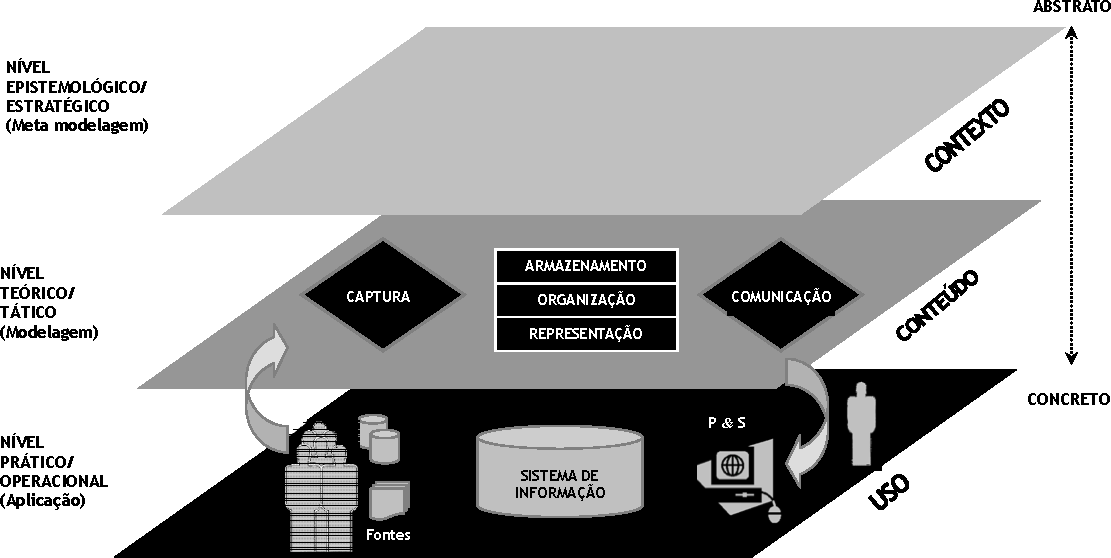
\includegraphics[scale=0.8]{imagens/fig_modeloAIMacedo.pdf}
  	\caption{\label{fig_m3hier}Metodologia de Meta-Modelagem (M{$^3$}):
  	hierarquia de sistemas de investigação}
  	\caption*{Fonte: \citeonline[p. 74]{van86}} 
\end{center} 
\end{figure}

A \autoref{tab-nivinv}\ldots

\begin{table}[htb]
\footnotesize
\caption[Níveis de investigação]{\footnotesize{Níveis de investigação.
\cite{van86}}}
\label{tab-nivinv}
\begin{tabular}{p{2.6cm}|p{6.0cm}|p{2.25cm}|p{3.40cm}}
  %\hline
   \textbf{Nível de Investigação} & \textbf{Insumos}  & \textbf{Sistemas de Investigação}  & \textbf{Produtos}  \\
    \hline
    Meta-nível & Filosofia da Ciência  & Epistemologia & Paradigma  \\
    \hline
    Nível do objeto & Paradigmas do metanível e evidências do nível inferior &
    Ciência  & Teorias e modelos \\
    \hline
    Nível inferior & Modelos e métodos do nível do objeto e problemas do nível inferior & Prática & Solução de problemas  \\
   % \hline
\end{tabular}
\end{table}


%---------------------------------------------------------------------
\section{Fontes de pesquisa} \label{metodologiaFontes}
%---------------------------------------------------------------------

A revisão da literatura foi realizada principalmente nas --- mas não limitada às
--- fontes seguintes:

\textbf{Bancos de Testes e Dissertações}

\begin{list}{--}{\parsep0.0cm\leftmargin2.0cm}
  \item Banco de Teses da CAPES (\url{http://www.capes.gov.br/servicos/banco-de-teses/});
  \item Banco de Teses e Dissertações da UnB (\url{http://bce.unb.br/});
\end{list}

\textbf{Bases de Dados}

\begin{list}{--}{\parsep0.0cm\leftmargin2.0cm}
  \item ACM Digital Library (\url{http://dl.acm.org/});
  \item Periódicos CAPES (\url{http://www.periodicos.capes.gov.br/})
  \item ProQuest (\url{http://search.proquest.com/})
  \item School of Information (\url{http://www.ischool.utexas.edu/});
  \item Web of Knowledge (\url{http://wok.mimas.ac.uk/});
  \item \ldots
\end{list}

\textbf{Periódicos}

\begin{list}{--}{\parsep0.0cm\leftmargin2.0cm}
  \item Ciência da Informação (IBICT);
  \item Journal of the American Society for Information Science and Technology
  (JA-SIST);
\end{list}

%---------------------------------------------------------------------
%---------------------------------------------------------------------
\subsection{Bibliometria}\label{metodologiaBibliometria}
%---------------------------------------------------------------------

A \autoref{tab_bibliometria_termosInformationConfig} contém dados bibliométricos
de pesquisas de termos chaves em algumas das bases de dados listadas na
\autoref{metodologiaFontes}\ldots

% EXEMPLO DE LONG TABLE
% INFORMATION e CONFIGURATION - Tabela principal de consultas de
\begin{center}
\footnotesize{
\begin{ThreePartTable}

\begin{longtable}{p{7.2cm}|p{6.3cm}|p{1.8cm}}

\caption[Resultados obtidos na consulta de termos ``configuration'' e
``information'' em bases de dados em 29.1.2012.]{\footnotesize{Resultados obtidos
na consulta de termos ``configuration'' e ``information'' em bases de dados.
Consultas realizadas em 29.1.2012. Período pesquisado: todos disponíveis nas
bases.}}
\label{tab_bibliometria_termosInformationConfig}
\\

%This is the header for the first page of the table...
\hline 
\textbf{Base de dados}	& \textbf{Termos e critérios} & \textbf{Resultados} \\
\hline 
%\endfirsthead
\endhead

%This is the footer for all pages except the last page of the table...
  \multicolumn{3}{r}{{Continua\ldots\ldots}} \\
\endfoot

%This is the footer for the last page of the table...
\hline \hline
\endlastfoot

%Now the data...

    % ``information configuration''
	\multirow{2}{*}{Academic Search Premier - ASP (EBSCO)}\tnote{a}
	& Titulo=(``information configuration'')
	& 1\tnote{b}
	\\
	& Titulo=(``configuration of information'')
	& 1\tnote{e}	
	\\ \hline	

	\multirow{2}{*}{Cambridge Journals Online}\tnote{a}
	& Titulo=(``information configuration'')
	& 0
	\\
	& Titulo=(``configuration of information'')
	& 0
	\\ \hline	

	\multirow{2}{*}{Highwire Press}\tnote{a}
	& Titulo=(``information configuration'')
	& 0
	\\
	& Titulo=(``configuration of information'')
	& 0
	\\ \hline	

	\multirow{2}{*}{Nature (NPG)}\tnote{a}
	& Titulo=(``information configuration'')
	& 0
	\\
	& Titulo=(``configuration of information'')
	& 0
	\\ \hline	

	\multirow{2}{*}{Oxford Journals (Oxford University Press)}\tnote{a}
	& Titulo=(``information configuration'')
	& 0
	\\
	& Titulo=(``configuration of information'')
	& 0
	\\ \hline	

	\multirow{3}{*}{SciELO.ORG}\tnote{a}
	& Titulo=(``information configuration'')
	& 0
	\\
	& Titulo=(``configuration of information'')
	& 0
	\\
	& Title: ``configuração da informação''
	& 0
	\\ \hline	

	\multirow{2}{*}{Science (AAAS)}\tnote{a}
	& Titulo=(``information configuration'')
	& 0
	\\
	& Titulo=(``configuration of information'')
	& 0
	\\ \hline	

	\multirow{2}{*}{ScienceDirect (Elsevier)}\tnote{a}
	& Titulo=(``information configuration'')
	& 0
	\\
	& Titulo=(``configuration of information'')
	& 0
	\\ \hline	

	\multirow{2}{*}{SpringerLink (MetaPress)}\tnote{a}
	& Titulo=(``information configuration'')
	& 0
	\\
	& Titulo=(``configuration of information'')
	& 0
	\\ \hline	

	\multirow{2}{*}{E-LIS}
	& Title: ``information configuration''
	& 2\tnote{c}
	\\
	& Title: ``configuration of information''
	& 1\tnote{d}
	\\ \hline	

	\multirow{2}{*}{Web of Knowledge}
	& Title: ``information configuration''
	& 0
	\\
	& Title: ``configuration of information''
	& 0
	\\ \hline	
	
\end{longtable}

	\begin{tablenotes}
		\item [a] Base de Periódicos CAPES.
		\item [b] O único texto obtido \ldots
		\item [c] Os textos recuperados \cite{hammer2005} e \cite{apps2001} se
		referem, respectivamente, a um manual de uso de uma ferramenta de
		gerenciamento de informação para bibliotecários e a um serviço baseado em Dublincore.
		\item [d] O único texto obtido \ldots
		\item [e] O único texto obtido \ldots

	\end{tablenotes}
	
\end{ThreePartTable}
}
\end{center}


% Figura - Web of Science 1 - Detalhamento
\begin{figure}[htb]
\begin{center}
  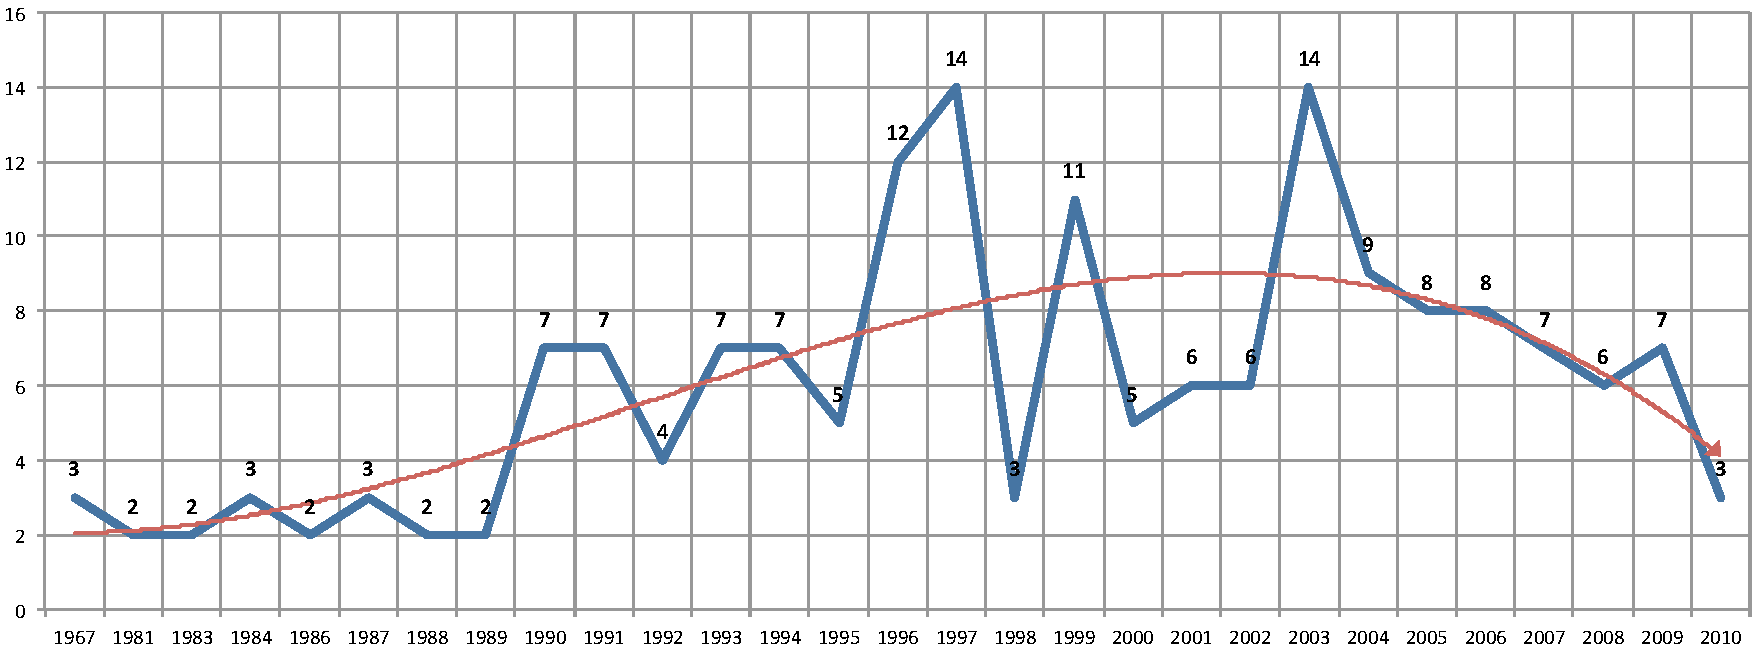
\includegraphics[scale=0.55]{imagens/bibliometriaWebOfScience1.pdf}
  \caption{\label{fig_biblioWebOfScience1}Bibliometria - Web of Science -
  Detalhamento da consulta - Critério: Title=(``configuration management'').}
  \caption*{Fonte: autores}
\end{center}
\end{figure}


%---------------------------------------------------------------------
